%!TEX root = ../thesis.tex
% Models in Astronomy

\chapter{Models of atmospheres and stars}
Synthetic stellar spectra {PHOENIX-ACES} and {BT-Settl} as well as atmopsheric spectra using {TAPAS}.


\textbf{earths atmopshere in the nir}

\textbf{Tapas models}



\textbf{Stellar models.}



\textbf{Evolution models.}


Models help us to understand model, fit and predict the measurements and results and allow to compare to reality.


%!TEX root = ../../thesis.tex


\section{Telluric correction}
\label{sec:telluric_correction}

\subsection{Earth's atmosphere}
\todo{move out of intro}
While the Earth's atmosphere is important for an Astronomer's lungs, it can be a nuisance for their ground-based observations.
As light form astronomical sources passes through the atmosphere, its molecular components absorb some of the light, changing spectral components observed by imprinting a transmission spectrum of our atmosphere.
The \ce{H2O} absorption is a key example as it defines the photometric and spectroscopic bands in the \nir{}. \missingfigure{example to point to}.

The correction of observations from the contamination of Earth's atmosphere is a complex process.\textbf{
    The transmission is variable on many different time scales, the water vapour change is rapid, concentrations of atmospheric constituents, to seasonal and longer.}
Such as the increase in atmospheric \ce{CO2} causing anthropamorphic climate change this requires 6\% change to \ce{CO2} line depths since 2000 Molecfit paper?
There is also variation with airmass, which depends on the observation angle in the sky and changes as targets move across the sky during the night.

other constituents, \ce{CO}, \ce{CO2}, \ce{CH4} \ldots{}, angle of observations.

An important consideration in detecting the constituents of planetary atmospheres is the characterization and removal of Earth's telluric lines.

e.g.\ 50\% error in \ce{CO2} detection on Mars atmosphere


Recently~\citet{ulmer-moll_telluric_2018} compared the telluric correction possible from three different synthetic telluric software against the standard star model.
Molecfit, a software from ESO was the most.

This is a growing field and there are other software available too\ldots{}


Water vapour content has rapid variability.
Works such as \citet{snellen_orbital_2010}, fit and remove the telluric variation during a series of observations\footnote{51 spectrum of the same target in 180 minutes for \citet{snellen_orbital_2010}}, to remove telluric lines and detect the absorption lines of exoplanet atmospheres.

\todo{finish this}


Telluric absorption map
\begin{figure}
    \centering
    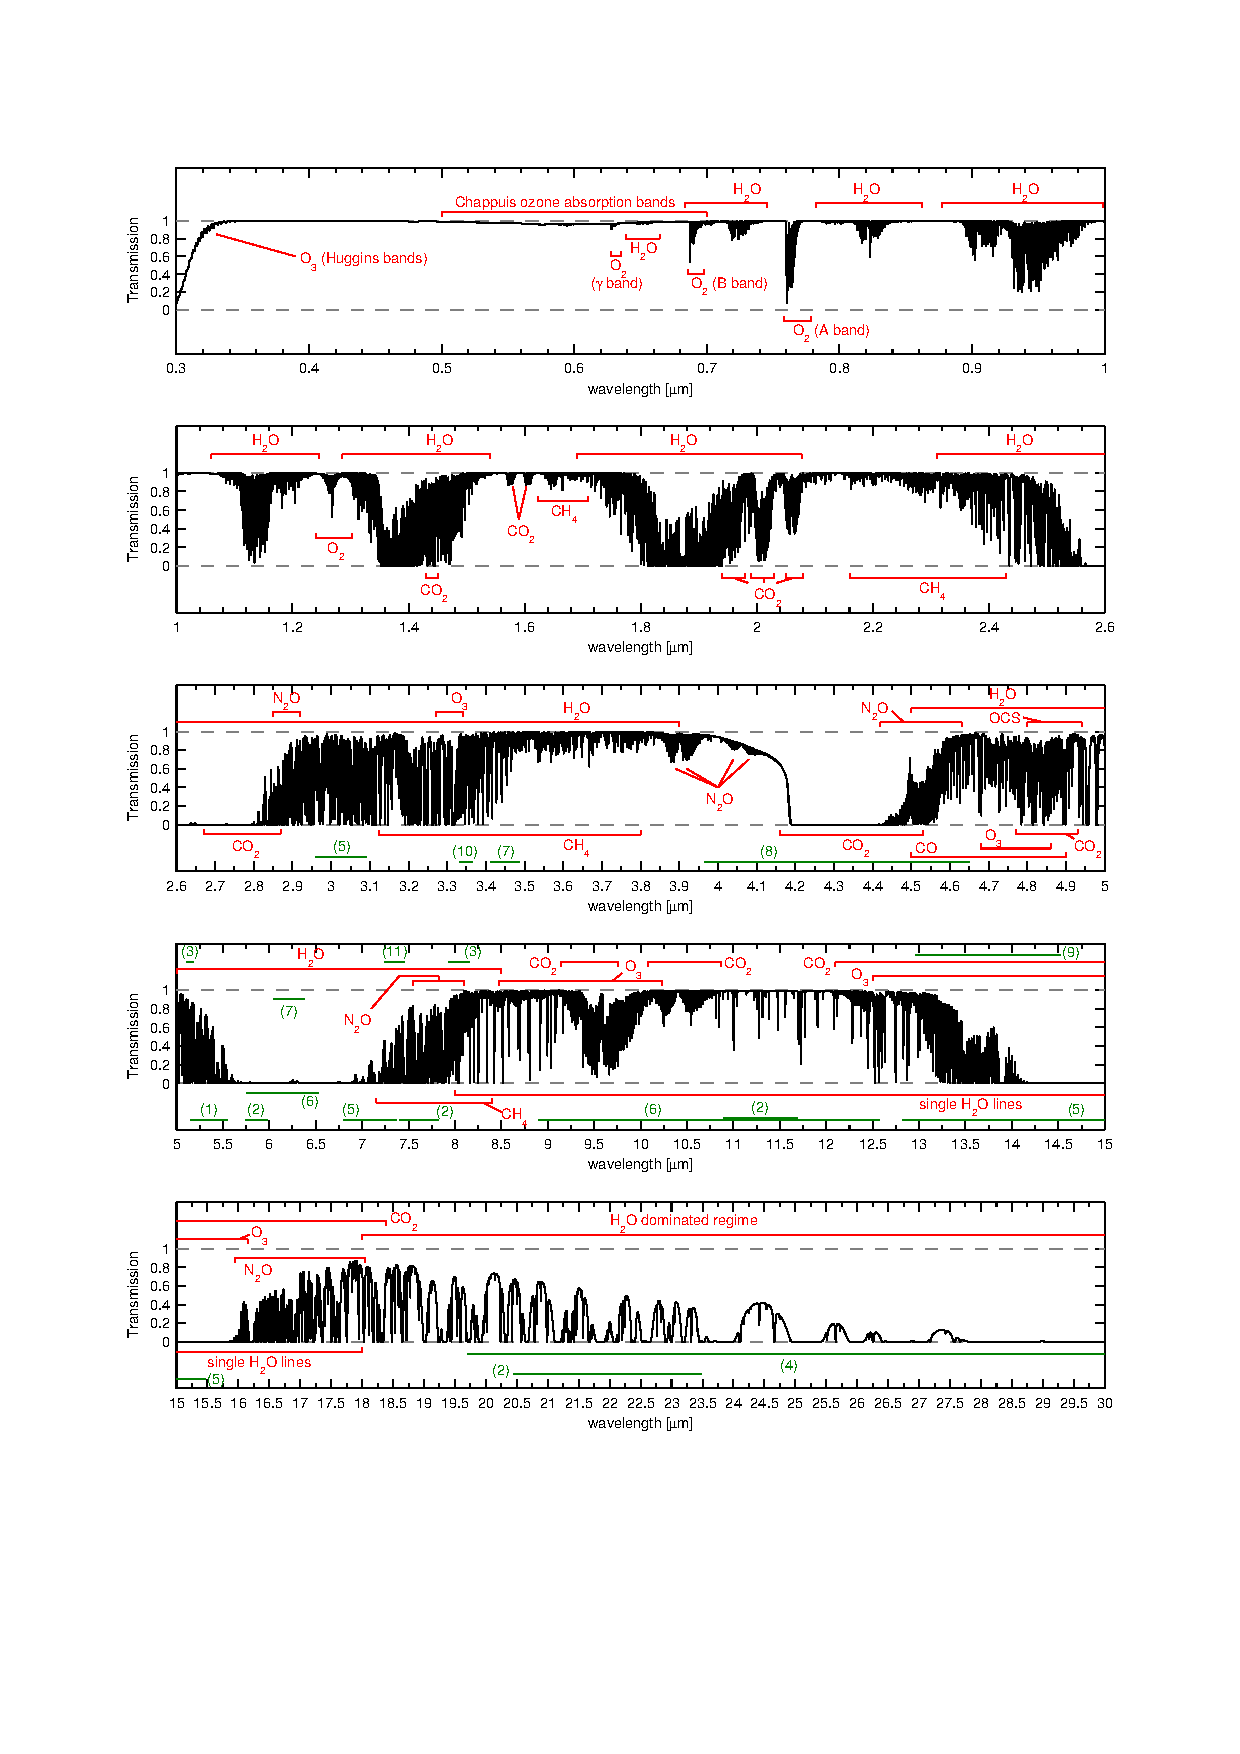
\includegraphics[width=0.9\linewidth]{figures/models/cropped_molecfit_absorbtion}
    \caption{Reproduction of Figure~1 of~\citet{smette_molecfit_2015} showing telluric absorption form 0.30 \um.
        Original caption:\textbf{add more here}}
    \label{fig:croppedmolecfitabsorbtion}
\end{figure}
\todo{Add original caption to~\cref{fig:croppedmolecfitabsorbtion}}




\subsection{Telluric models}

Utilizing telluric models has been shown to be better than the standard star method.
\subsubsection{TAPAS}
\label{subsubsec:TAPAS}

\subsection{Tapas models}
\todo{ADAPT THis section to explain the models more generally.
    Move the usage back to Reduction section}
\label{subsec:tapas_models}
For the wavelength calibration and telluric correction methods we use telluric line models.
These have been show to provide as good or better telluric correction compared to the telluric standard method \reference{telluric model correction methods original}and~\citep{ulmer-moll_telluric_2018}.

We utilized the {TAPAS} (Transmissions of the AtmosPhere for AStronomical data) web-service\footnote{\href{http://www.pole-ether.fr/tapas/}{http://www.pole-ether.fr/tapas/}}~\citep{bertaux_tapas_2014} to obtain atmospheric transmission models for each observation. {TAPAS} uses the standard line-by-line radiative transfer model code LBLRTM~\citep{clough_linebyline_1995} along with the 2008 {HITRAN} spectroscopic database~\citep{rothman_hitran_2009} and {ARLETTY} atmospheric profiles derived using meteorological measurements from the {ETHER} data center\footnote{\href{http://www.pole-ether.fr}{http://www.pole-ether.fr}} to create telluric line models.

The {ARLETTY} atmospheric profiles have a 6 hour resolution, so there may be a slight difference between the actual profile at the time of observation.

We use the mid-observation time to retrieve transmission models for each observation, with the {ARLETTY} atmospheric profiles\footnote{Nearest of the 6 hourly profiles} and vacuum wavelengths selected.
The telluric models were retrieved without any barycentric correction to keep the telluric lines at a radial velocity of zero with respect to the instrument.

{TAPAS} allows for the choice of atmospheric constituents included in the model spectra.
We obtained one model with all available species present, convolved to a resolution of \(\rm R=50\,000\), and another two models without an instrumental profile convolution applied.
For these two extra models, one contained only the transmission spectra of \ce{H2O} while the other contained all other constituents except \ce{H2O}.
This was to explore a known issue with the depth of \ce{H2O} absorption lines in the {TAPAS}~\citet{bertaux_tapas_2014}. \cref{subsec:telluric_correction}.


\todo{Look at} -> synthesizing telluric spectra \nir{} for {CRIRES}~\cite{seifahrt_synthesising_2010}

Using {TAPAS} is contrasted alongside Molecfit and Telfit in~\cite{ulmer-moll_telluric_2018}.
We conclude that \ldots



%!TEX root = ../../thesis.tex

\section{Synthetic Stellar models}:

In the work we make extensive use of the {PHOENIX-ACES} models with some experimentation with the {BT-Settl} models.
A collection of several theoretical stellar spectral libraries can be found at Spanish Virtual Observatory \href{http://svo2.cab.inta-csic.es/theory/newov/index.php}{Theoretical Spectra Web Server}.



\subsection{PHOENIX-ACES}

Available \todo{FINISH}




\subsection{BT-Settl}

Available \todo{FINISH}

Harder to work with.

Other models which have not been used here.
Kruz models a directory of different model can be found \ldots{}?

BT-Settl have less but are suitable for BDs.
We did not extend below the {PHOENIX-ACES} lower temperature of 2300\K{}




\section{Evolutionary models}
Baraffe evolutionary models.
\todo{Example from their paper of evolutionary tracks or something}


\section{Estimating Companion-host Flux ratio}
\label{sec:compaion_flux_ratio}
In order to visually or spectroscopically detect binary or planetary companions it is helpful to calculate the flux/contrast ratio between the host and companion.

The companion-host flux or contrast ratio of the system can be estimated using:
\begin{equation}
\frac{F_{2}}{F_{1}} \approx 2.512^{m_{1} - m_{2}}, \label{eqn:mag_flux_ratios}
\end{equation}
where \(m_{1}\) and \(m_{2}\) are the magnitude of the host and companion respectively.

The photometric apparent magnitudes for the host stars, \(m_{1}\), in several wavelength bands are easily obtained through online catalogues such as {SIMBAD}~\citep{wenger_simbad_2000} or {2MASS} \citep{skrutskie_two_2006}.
However, the magnitudes of the companions, \(m_{2}\), are not readily available as they have not been directly measured.
Stellar evolution models of \citet{baraffe_evolutionary_2003, baraffe_new_2015} are used to estimate the magnitude of the companion.
These models tabulate several properties of low-mass stars and BDs during their evolution.
These include the temperature, radius, luminosity, and absolute magnitudes in several photometric bands, for a range of companion masses and stellar ages.
A given companion mass, and a stellar age will uniquely identify a point in the Baraffe models which corresponds to a specific magnitude for the companion.
The tables provided in \citet{baraffe_evolutionary_2003, baraffe_new_2015} are also interpolated to reach companion masses and stellar ages between the models provided.

In \cref{tab:estimated_flux_ratios} the host-companion flux ratio estimates for the targets analysed in this work are presented. The {K}-band flux ratios are calculated to match the observed {CRIRES} spectra at 2.1\um{}. The stellar ages used for the each system are given in \cref{tab:starparams} while the companion masses are given from \cref{tab:orbitparams}. The age and companion mass are both used to obtain the absolute magnitude for the companions. For the companions in which only the minimum mass (\mtwosini{}) is known then the flux-ratio given will be the lower limit, or worst case scenario.

%!TEX root = ../../thesis.tex
\begin{table*}
    \small
    \centering
    \begin{threeparttable}[b]
        \caption{Estimated flux ratios given the companion mass (\(\textrm{M}_{2}\) or \(\textrm{M}_{2} \sin{i}\)) from \tref{tab:orbitparams}.} 
        \begin{tabular}{l c c c c c c}%[hb]
            \toprule
            & Host& & Host & Companion & Estimated & Estimated  \\  % 2017
            Companion & $m_{K}$ & $\pi$ & M\(_{K}\) & M\(_{K}\) & \(\rm F_{2}/F_{1} \) & \(\rm N_{2}/N_{1} \) \\
            & & mas & & & \textit{K}-band &  (noise ratio) \\
            \midrule
            {HD 4747} & 5.305 & 53.184 & 3.82 & 14.17 & \(7\times10^{-5} \) & 76 \\  % 2017
            {HD 162020} & 6.539 & 32.410 & 4.10 & 23.36 & \(2\times10^{-8} \) & 1\,615 \\  %
            {HD 167665} & 5.038 & 32.014 & 2.60 & 13.21 & \(6\times10^{-5} \) & 105 \\  %  -- \(2\times10^{-5} \)  best case based on age rage.
            {HD 168443b} & 5.211 & 25.208 & 2.35 & 42.19 & \(1\times10^{-16} \) & \(1\times10^{8} \) \\ 
            {HD 168443c} & 5.211 & 25.208 & 2.35 & 29.55 & \(1\times10^{-11} \) & \(4\times10^{5} \) \\  %(c)
            {HD 202206}B & 6.485\tnote{a}& 21.726 & 3.04 & 21.63 & \(4\times10^{-8} \) & 1\,586 \\  %(B)   % May2017
            {HD 202206}c & 6.485\tnote{a}& 21.726 & 3.04 & 45.63 & \(9\times10^{-18}\) & \(2\times10^{7} \) \\  %(B)   % May2017
            {HD 211847}B & 7.018 & 20.489 & 3.50 & 8.40 & 0.011 & 14 \\  %B % 2017
            {HD 30501} & 5.525 & 49.081 & 3.96 & 10.38 & 0.003 & 27 \\
            \bottomrule
        \end{tabular}\label{tab:estimated_flux_ratios}
        \begin{tablenotes}
            \item  [a]{Magnitude from {2MASS} catalogue instead of {SIMBAD}.}
        \end{tablenotes}
    \end{threeparttable}

\end{table*} % \label{tab:estimated_flux_ratios}

The magnitudes provided by {SIMBAD} are given in apparent magnitude, $m$, while the magnitudes in the evolutionary models are absolute magnitudes $M$. That is, the apparent magnitude that the star would have if it was observed at a distance of 10 parsecs (32.6 light-years). The apparent magnitudes of the hosts are converted to absolute magnitudes using \(M = m - \mu\) where \(\mu\) is the distance modulus:
\begin{equation}
\mu = 5 \log_{10}(d_{pc}) -5. \label{eqn:distance_modulus}
\end{equation}
Here $d_{pc}$ is the distance to the object in parsec. The distance is obtained from the trigonometric parallax  $\pi$ using the formula $d(pc) = 1 /\pi(arcsec)$, with the parallax in arcseconds\footnote{Most parallax values e.g.\ GAIA are tabulated in milliarcseconds (mas). Therefore it is important to remember to convert the parallax to arcseconds first, to avoid embarrassing calculation errors!}. In this work the recent high-precision parallax measurements from GAIA are used~\citet{collaboration_gaia_2018}.

From the flux ratio the noise ratio between the host and companion can also be calculated in a similar way using the equation \(N_{2}/N_{1} = \sqrt{2} \times\sqrt{F_{1}/F_{2}}\).

\todo{this section is completed i think}

\subsubsection{Baraffe tables}
\label{subsubsec:baraffe_tables_code}
A simple tool\footnote{Available at \href{https://github.com/jason-neal/baraffe_tables}{https://github.com/jason-neal/baraffe\_tables}} was created to calculate/estimate the host-companion flux ratio using the~\citet{baraffe_evolutionary_2003, baraffe_new_2015} evolution tables.
Given the name of the target star, the mass of a companion and the stellar/system age the tool determines the flux ratios in the available spectral bands.
The tool uses the targets name to query\href{https://zenodo.org/record/1160627}{\emph{astroquery} package} the {SIMBAD} database to obtain the stellar properties, specifically the flux magnitudes and parallax. It then interpolates the Baraffe tables to the desired companion mass and age, calculating and returning values for all parameters of the companion given in the tables (e.g.\ \(\teff\), \logg, \(R/R_{\odot}\)).
The stellar magnitudes are converted to absolute values using \cref{eqn:distance_modulus} and the flux ratios computed using \cref{eqn:mag_flux_ratios}.

An extension of this tool is that can be used to perform the reverse calculation also. That is, given the target name, age and flux ratio in a given band it can estimate the mass of the companion mass using the evolution tables.

\todo{This section is completed I think}
